

\documentclass{article}
\input{myheader.tex}
\graphicspath{ {img/} }
\title{Phone Book Data Structure
\\
~\\\small{All the phone numbers in the world in 2.5 GigaBytes}}
\author{Pratik Deoghare}
\begin{document}
\maketitle
\tableofcontents

\section{Problem}

A phone company wants to keep track of subscribers to their service. They want
to be able to perform following operations, 

\begin{enumerate}
    \item Assign new customer a phone number that is not already in use.
    \item Remove customer from the database and make his number available. 
    \item Find an unused number to assign to a new customer.
\end{enumerate}

Range of phone numbers is 000-000-0000 to 999-999-9999.

\newpage
\section{Solution}

We can store all the numbers at nodes of a binary tree arranged as shown in
figures. Each node has three things associated with it, 

\begin{enumerate}
    \item Number 
    \item Is this number in use? 
    \item Are all the descendents of this node in use? (Node
        is colored red if this is true).
\end{enumerate}


Let $n$ be the number of subscribers. 

To add a subscriber mark it as in use and update color of its ancestors. 
To remove a subscriber mark it as not in use and update color of its ancestors. 
Since node cannot have more than $\log n$ ancestors these operations take $O(\log n)$.

To find an available number start at the root and follow the path avoiding red
nodes down the tree until an unused node is found. Since red colored node means
all its descendents are in use searching its subtrees can be avoided. This operation
is $O(\log n)$. 

To check if a number is in use we can climb down the tree upto the number and check if 
its in use. This takes $O(\log n)$.

Now trivial implementation of this needs space for $n$ numbers and two booleans
per number. So $n \log n + 2 n$ bits. To manage all 10 digit numbers this is
roughly 44 Gigabytes without counting the space required to store pointers
between the nodes ofthe tree. 

Fortunately, this tree has special structure. Its a min heap. We can store min
heap as array where, index of left child of $i$ is given by $2i + 1$ and right
child by $2i +2$ assuming 0 based indexing. And index of parent node of $i$ is
given by $\lfloor i /2 \rfloor$ if $i$ is odd and by $i/2 - 1$ if $i$ is even. 

Since all the numbers between 0 to $n$ are present we can arrange them such
that index of the number matches the number. Hence we don't have to store the
numbers themselves. All we need to store is information about if the number is
in use and are all the descendents of it are in use. This information can be
stored as 2 arrays of $n$ bits each. This requires only 2.5 Gigabytes of space. 

Since $i^{th}$ entry in the array has information about number $i$. We can
check if the number is in use in $O(1)$. 

Please see the code for implementation details. 

\begin{figure}[H]
    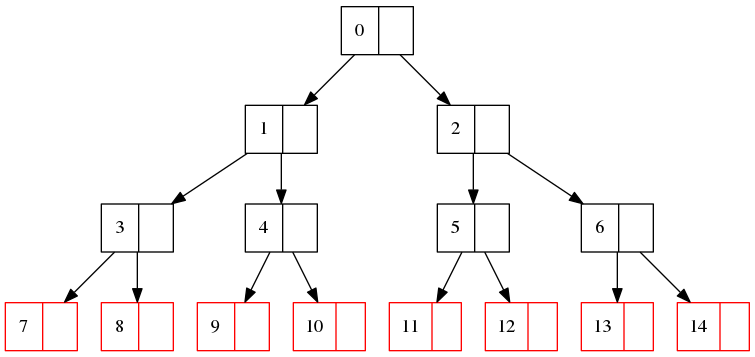
\includegraphics[width=\textwidth]{init}
    \caption{Initial setup}
    \label{fig:init}
\end{figure}

\begin{figure}[H]
    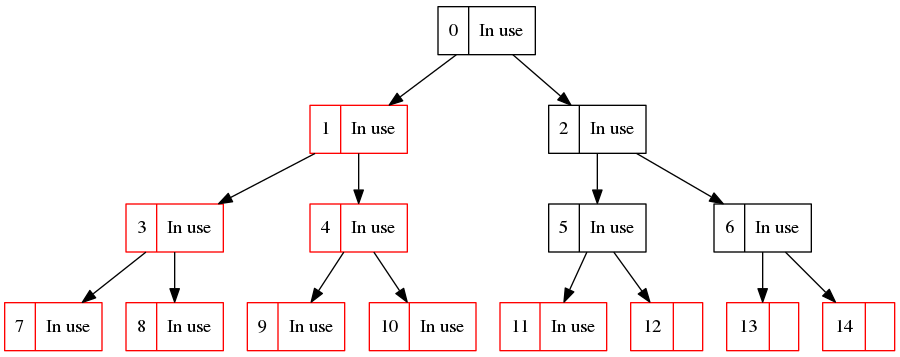
\includegraphics[width=\textwidth]{addupto11}
    \caption{After adding subscribers for numbers from 0 to 11}
    \label{fig:addupto11}
\end{figure}

\begin{figure}[H]
    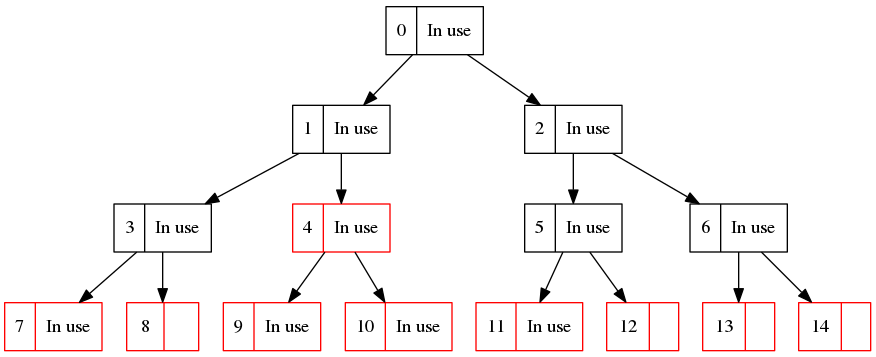
\includegraphics[width=\textwidth]{minuseight}
    \caption{Subscriber 8 unsubscribes}
    \label{fig:minuseight}
\end{figure}


\newpage
\section{Usage}

\begin{verbatim}

#include "PhoneBook.h"

int main(){
    my::PhoneBook<9999999999> pb;
    ...
    pb.is_used(number); // Check if number is used. 
    pb.set_used_status(number, true); // Add user 
    pb.set_used_status(number, false); // Remove user 
    pb.get_unused(); // Get an unused number 

    ...
}

\end{verbatim}


Find code in \texttt{./code/}. 

Basic test code in \texttt{./code/test.cc}. 

Valgrind output: 


\begin{verbatim}
λ ~/code/phonebook/code/ master* valgrind ./bigtest
==22343== Memcheck, a memory error detector
==22343== Copyright (C) 2002-2013, and GNU GPL'd, by Julian Seward et al.
==22343== Using Valgrind-3.9.0 and LibVEX; rerun with -h for copyright info
==22343== Command: ./bigtest
==22343== 
==22343== Warning: set address range perms: large range [0x39fe1040, 0x847f8cc0) (undefined)
==22343== Warning: set address range perms: large range [0x847f9040, 0xcf010cc0) (undefined)
==22343== Warning: set address range perms: large range [0x847f9028, 0xcf010cd8) (noaccess)
==22343== Warning: set address range perms: large range [0x39fe1028, 0x847f8cd8) (noaccess)
==22343== 
==22343== HEAP SUMMARY:
==22343==     in use at exit: 0 bytes in 0 blocks
==22343==   total heap usage: 2 allocs, 2 frees, 2,500,000,000 bytes allocated
==22343== 
==22343== All heap blocks were freed -- no leaks are possible
==22343== 
==22343== For counts of detected and suppressed errors, rerun with: -v
==22343== ERROR SUMMARY: 0 errors from 0 contexts (suppressed: 2 from 2)
λ ~/code/phonebook/code/ master* 

\end{verbatim}





\end{document}

